% This header creates a tabular view on the left
% and an elevation profile on the right header side
%
% DEFAULT SKITOUR HEADER
%
% create header
\ohead[\mydate]{}
\ohead[\mydate]{}
\graphicspath{{\mypath/}}
\cfoot[\vspace{-0.7em}  \myregion ]{}
\ifoot[{\vspace{-2.7em} \includegraphics[scale=0.2]{meta/parkplatz/\myparking} }]{}
\ofoot[\vspace{-0.7em}  \myseason $~\bullet$ S. \pagemark ]{}

% create elevation profile
\AddToShipoutPicture*{
	\AtTextUpperLeft{
		\put(\myhtx,\myhty){
			\parbox[b][\paperheight]{\textwidth}{
				\raggedleft
				\adjustbox{max height=5.0cm, max width=.65\textwidth,keepaspectratio}{
					% GNUPLOT: LaTeX picture with Postscript
\begingroup
  \makeatletter
  \providecommand\color[2][]{%
    \GenericError{(gnuplot) \space\space\space\@spaces}{%
      Package color not loaded in conjunction with
      terminal option `colourtext'%
    }{See the gnuplot documentation for explanation.%
    }{Either use 'blacktext' in gnuplot or load the package
      color.sty in LaTeX.}%
    \renewcommand\color[2][]{}%
  }%
  \providecommand\includegraphics[2][]{%
    \GenericError{(gnuplot) \space\space\space\@spaces}{%
      Package graphicx or graphics not loaded%
    }{See the gnuplot documentation for explanation.%
    }{The gnuplot epslatex terminal needs graphicx.sty or graphics.sty.}%
    \renewcommand\includegraphics[2][]{}%
  }%
  \providecommand\rotatebox[2]{#2}%
  \@ifundefined{ifGPcolor}{%
    \newif\ifGPcolor
    \GPcolortrue
  }{}%
  \@ifundefined{ifGPblacktext}{%
    \newif\ifGPblacktext
    \GPblacktexttrue
  }{}%
  % define a \g@addto@macro without @ in the name:
  \let\gplgaddtomacro\g@addto@macro
  % define empty templates for all commands taking text:
  \gdef\gplbacktext{}%
  \gdef\gplfronttext{}%
  \makeatother
  \ifGPblacktext
    % no textcolor at all
    \def\colorrgb#1{}%
    \def\colorgray#1{}%
  \else
    % gray or color?
    \ifGPcolor
      \def\colorrgb#1{\color[rgb]{#1}}%
      \def\colorgray#1{\color[gray]{#1}}%
      \expandafter\def\csname LTw\endcsname{\color{white}}%
      \expandafter\def\csname LTb\endcsname{\color{black}}%
      \expandafter\def\csname LTa\endcsname{\color{black}}%
      \expandafter\def\csname LT0\endcsname{\color[rgb]{1,0,0}}%
      \expandafter\def\csname LT1\endcsname{\color[rgb]{0,1,0}}%
      \expandafter\def\csname LT2\endcsname{\color[rgb]{0,0,1}}%
      \expandafter\def\csname LT3\endcsname{\color[rgb]{1,0,1}}%
      \expandafter\def\csname LT4\endcsname{\color[rgb]{0,1,1}}%
      \expandafter\def\csname LT5\endcsname{\color[rgb]{1,1,0}}%
      \expandafter\def\csname LT6\endcsname{\color[rgb]{0,0,0}}%
      \expandafter\def\csname LT7\endcsname{\color[rgb]{1,0.3,0}}%
      \expandafter\def\csname LT8\endcsname{\color[rgb]{0.5,0.5,0.5}}%
    \else
      % gray
      \def\colorrgb#1{\color{black}}%
      \def\colorgray#1{\color[gray]{#1}}%
      \expandafter\def\csname LTw\endcsname{\color{white}}%
      \expandafter\def\csname LTb\endcsname{\color{black}}%
      \expandafter\def\csname LTa\endcsname{\color{black}}%
      \expandafter\def\csname LT0\endcsname{\color{black}}%
      \expandafter\def\csname LT1\endcsname{\color{black}}%
      \expandafter\def\csname LT2\endcsname{\color{black}}%
      \expandafter\def\csname LT3\endcsname{\color{black}}%
      \expandafter\def\csname LT4\endcsname{\color{black}}%
      \expandafter\def\csname LT5\endcsname{\color{black}}%
      \expandafter\def\csname LT6\endcsname{\color{black}}%
      \expandafter\def\csname LT7\endcsname{\color{black}}%
      \expandafter\def\csname LT8\endcsname{\color{black}}%
    \fi
  \fi
    \setlength{\unitlength}{0.0500bp}%
    \ifx\gptboxheight\undefined%
      \newlength{\gptboxheight}%
      \newlength{\gptboxwidth}%
      \newsavebox{\gptboxtext}%
    \fi%
    \setlength{\fboxrule}{0.5pt}%
    \setlength{\fboxsep}{1pt}%
\begin{picture}(9680.00,4800.00)%
    \gplgaddtomacro\gplbacktext{%
      \colorrgb{0.00,0.00,0.00}%
      \put(222,159){\makebox(0,0){\strut{}0\scriptsize km}}%
      \colorrgb{0.00,0.00,0.00}%
      \put(3346,159){\makebox(0,0){\strut{}5\scriptsize km}}%
      \colorrgb{0.00,0.00,0.00}%
      \put(6470,159){\makebox(0,0){\strut{}10\scriptsize km}}%
      \colorrgb{0.00,0.00,0.00}%
      \put(8700,620){\makebox(0,0)[l]{\strut{}1000\scriptsize m}}%
      \colorrgb{0.00,0.00,0.00}%
      \put(8700,1251){\makebox(0,0)[l]{\strut{}1200\scriptsize m}}%
      \colorrgb{0.00,0.00,0.00}%
      \put(8700,1883){\makebox(0,0)[l]{\strut{}1400\scriptsize m}}%
      \colorrgb{0.00,0.00,0.00}%
      \put(8700,2515){\makebox(0,0)[l]{\strut{}1600\scriptsize m}}%
      \colorrgb{0.00,0.00,0.00}%
      \put(8700,3146){\makebox(0,0)[l]{\strut{}1800\scriptsize m}}%
      \colorrgb{0.00,0.00,0.00}%
      \put(8700,3778){\makebox(0,0)[l]{\strut{}2000\scriptsize m}}%
      \colorrgb{0.00,0.00,0.00}%
      \put(8700,4410){\makebox(0,0)[l]{\strut{}2200\scriptsize m}}%
    }%
    \gplgaddtomacro\gplfronttext{%
      \csname LTb\endcsname%
      \put(4786,4699){\makebox(0,0)[l]{\strut{}\textcolor{skitour}{Kl. Daumen \tiny 2197m}}}%
    }%
    \gplgaddtomacro\gplbacktext{%
    }%
    \gplgaddtomacro\gplfronttext{%
    }%
    \gplbacktext
    \put(0,0){\includegraphics{hoehenprofil}}%
    \gplfronttext
  \end{picture}%
\endgroup

				}
			}
		}
	}
}

\def\arraystretch{1.3} % bessere Lesbarkeit im Kopfteil
\vspace{-0.75em}
{\small  \setstretch{1.3}
% left table
\begin{tabularx}{\headersize\textwidth}{X X X X X}
	\multicolumn{4}{c}{\rating}              \\
	$\uparrow$         \ascent   hm           &
	$\rightsquigarrow$ \distance km           &
	LLB                \LLB                  \\

	\rule{0pt}{3ex} $\vec{t}$ \movingtime h   &
	$\Delta t$                \overalltime h  &
	\Cross          \space    \summittime  h \\

	\clock\space    \starttime                &
	\multicolumn{2}{l}{ \smiley\space \pbox{2.8cm}{\scriptsize{ \comrades }}} \\

	\multicolumn{2}{c}{ \difficulty }         &
	% empty lines for difficulty
	                                          &
	                                         \\
	& \multicolumn{2}{c}{ \startpoint }

\vspace{0.5em}
\end{tabularx}
}\\

% create map
\begin{wrapfigure}[\mapwrap]{R}{\mapsize\textwidth}
	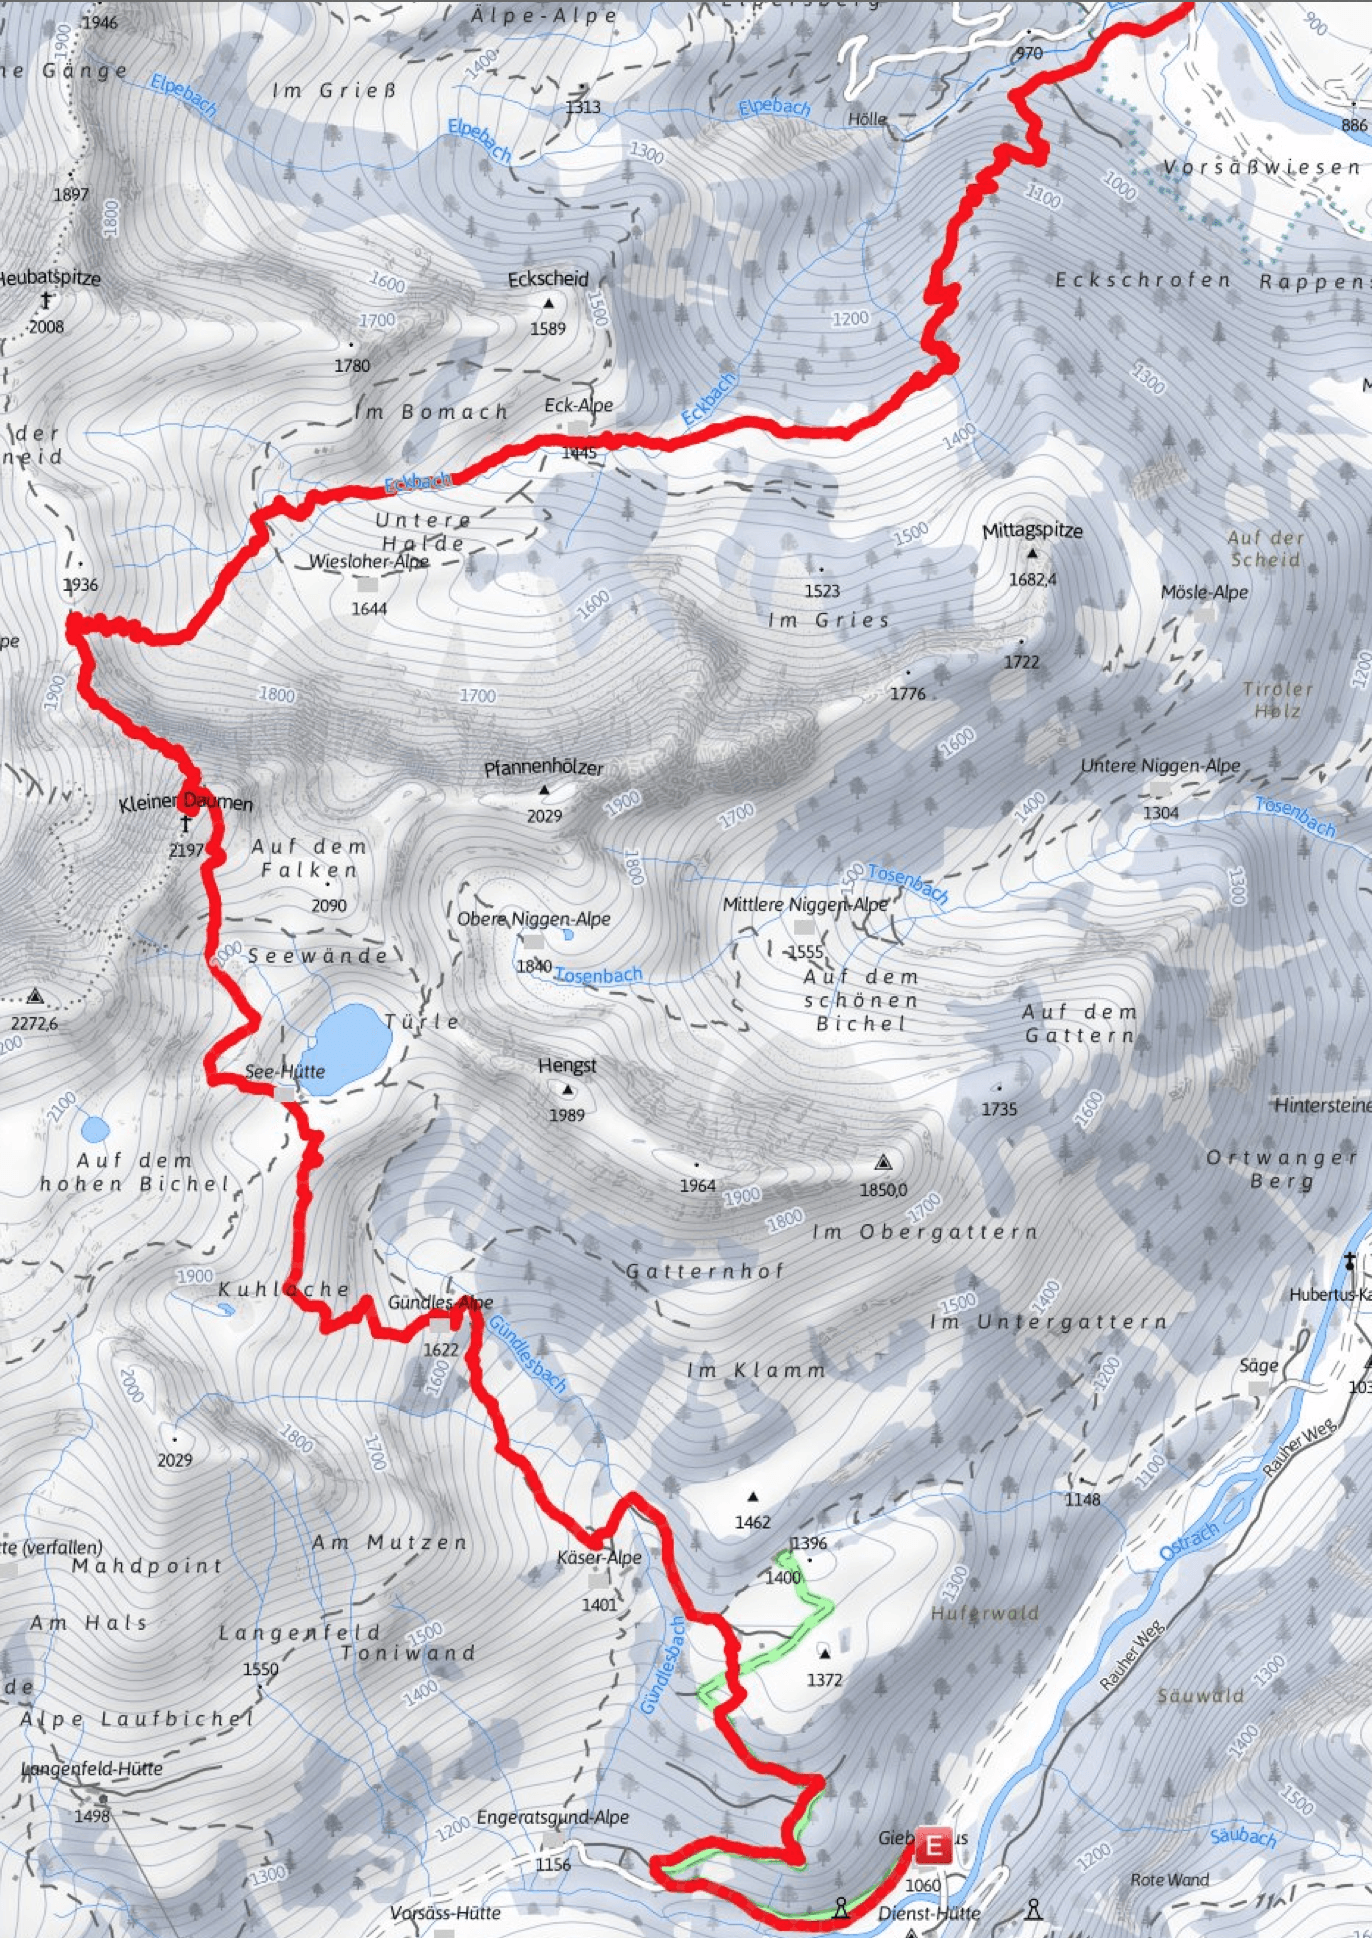
\includegraphics[width=\mapsize\textwidth]{karteninfo}
	\vspace{-0.7em}
\end{wrapfigure}
\setstretch{1.0}
